\documentclass[12pt,a4paper]{article}

\usepackage[utf8]{inputenc}
\usepackage[T1]{fontenc}
\usepackage{amsmath}
\usepackage{amsfonts}
\usepackage{amssymb}
\usepackage{graphicx}
\usepackage{float}
\usepackage{cite}
\usepackage{url}
\usepackage{geometry}
\usepackage{fancyhdr}
\usepackage{listings}
\usepackage{color}
\usepackage{subcaption}
\usepackage{physics}
\usepackage{xcolor}

\geometry{
    left=2.5cm,
    right=2.5cm,
    top=2.5cm,
    bottom=2.5cm
}

\pagestyle{fancy}
\fancyhf{}
\rhead{\thepage}
\lhead{Particle Motion in Electric Fields}

% Code listing settings
\lstset{
    language=Matlab,
    basicstyle=\footnotesize\ttfamily,
    keywordstyle=\color{blue},
    commentstyle=\color{green!50!black},
    stringstyle=\color{red},
    showstringspaces=false,
    breaklines=true,
    frame=single
}

% Color legend for the report
\definecolor{myblue}{RGB}{0,102,204}     % field lines
\definecolor{myyellow}{RGB}{242,207,74}  % electric field vectors
\definecolor{myred}{RGB}{204,0,0}        % equipotential lines
\definecolor{mycyan}{RGB}{0,204,204}     % zero potential

\title{
    Numerical Simulation of Charged Particle Motion in Electric Fields:\\
    A Computational Study of Trajectories and Field Interactions
}
\author{Hariton Marian}
\date{\today}

\begin{document}

\maketitle

\begin{abstract}
This report presents a numerical simulation study of charged particle motion in electric fields generated by multiple point charges. The implementation uses MATLAB and a modular codebase to visualize electric fields (field lines, equipotentials, and vector fields) and to simulate particle trajectories starting from the origin $(0,0)$. All particle motion simulations use the classical fourth-order Runge–Kutta (RK4) integrator with a fixed time step. The report documents the physical background, numerical methods, implementation details, and selected results for dipole, quadrupole, and line-charge configurations. Color conventions used in the visualizations are specified for reproducibility.
\end{abstract}

\tableofcontents
\newpage

\section{Introduction}
The dynamics of charged particles in electrostatic fields are foundational in classical electrodynamics and appear across many domains: beam dynamics, plasma physics, and electrostatic trapping. While some simple fields admit closed-form solutions, realistic multi-charge configurations generally do not, so numerical methods are essential. This project builds an interactive MATLAB toolkit for visualizing two-dimensional electric fields and simulating the motion of a small test particle placed at the origin with zero initial velocity.

\section{Theoretical Background}

\subsection{Coulomb's Law and Superposition}
The electric field $\vec{E}(\vec{r})$ due to $N$ point charges $q_i$ at positions $\vec{r}_i$ is:
\begin{equation}
    \vec{E}(\vec{r}) = \frac{1}{4\pi\epsilon_0}\sum_{i=1}^N \frac{q_i (\vec{r}-\vec{r}_i)}{|\vec{r}-\vec{r}_i|^3},
\end{equation}
with $\epsilon_0$ the permittivity of free space (and $k = 1/(4\pi\epsilon_0) \approx 8.99\times10^9\ \mathrm{N\,m^2/C^2}$).

In Cartesian coordinates for a 2D plane:
\begin{align}
    E_x(x,y) &= k \sum_{i=1}^N \frac{q_i (x - x_i)}{\left[(x-x_i)^2 + (y-y_i)^2\right]^{3/2}},\\
    E_y(x,y) &= k \sum_{i=1}^N \frac{q_i (y - y_i)}{\left[(x-x_i)^2 + (y-y_i)^2\right]^{3/2}}.
\end{align}

\subsection{Equations of Motion}
A test particle with charge $q$ and mass $m$ obeys Newton's second law in the presence of an electrostatic field:
\begin{equation}
    m\ddot{\vec{r}}(t) = q\,\vec{E}(\vec{r}(t)).
\end{equation}

Introducing velocity components, the second-order system becomes first order:
\begin{align}
    \dot{x} &= v_x,\quad \dot{y} = v_y,\\
    \dot{v}_x &= \frac{q}{m}E_x(x,y),\quad \dot{v}_y = \frac{q}{m}E_y(x,y).
\end{align}

\subsection{Energy Considerations}
The total mechanical energy (kinetic + potential) for a non-radiating classical test particle is:
\begin{equation}
    E_\text{total} = \frac{1}{2}m(v_x^2 + v_y^2) + q\,V(x,y),
\end{equation}
with the electrostatic potential
\begin{equation}
    V(x,y) = k\sum_{i=1}^N \frac{q_i}{\sqrt{(x-x_i)^2+(y-y_i)^2}}.
\end{equation}

In our numerical RK4 implementation, energy is monitored to check integration accuracy.

\section{Visualization Color Scheme}
For clarity and consistent interpretation, the visualization colors are:

\begin{itemize}
    \item \textbf{Field lines:} \textcolor{myblue}{Blue}
    \item \textbf{Electric field vectors (quiver):} \textcolor{myyellow}{Yellow}
    \item \textbf{Equipotential lines:} \textcolor{myred}{Red}
    \item \textbf{Zero potential contour:} \textcolor{mycyan}{Cyan}
    \item \textbf{Positive point charges:} Red markers with white ``+q'' label
    \item \textbf{Negative point charges:} Blue markers with white ``-q'' label
    \item \textbf{Simulated particle:} White filled circle; trajectory drawn as dashed white line
\end{itemize}

These conventions match the MATLAB colors used in the code (RGB triplets), so exported figures maintain consistent appearance.

\section{Numerical Methodology}

\subsection{Field Calculation}
Field components are computed pointwise using superposition. To avoid numerical singularities when evaluating very close to source charges, a small regularization radius $r_\text{min}$ is applied (e.g., $r_\text{min}=0.1$ m): distances smaller than $r_\text{min}$ are clamped to $r_\text{min}$ to prevent blow-up of $1/r^2$.

\subsection{Particle Integration: RK4 only}
All particle motion simulations use the classical \textbf{fourth-order Runge–Kutta} integrator (RK4). RK4 is chosen for its balance of accuracy and cost. The system state is $\mathbf{y} = [x, y, v_x, v_y]^T$ and the right-hand side $\mathbf{f}(\mathbf{y})$ is computed from the local electric field via the relation:
\[
    \mathbf{f}(\mathbf{y}) = 
    \begin{bmatrix} 
        v_x \\ v_y \\ \dfrac{q}{m}E_x(x,y) \\ \dfrac{q}{m}E_y(x,y)
    \end{bmatrix}.
\]
The RK4 update over a time step $\Delta t$ is applied in the standard way.

\subsection{Time Step and Stability}
A fixed time step is used throughout (no adaptive time stepping). Typical choices used in the simulations are:
\[
    \Delta t = 1\times 10^{-6}\ \mathrm{s}\ \text{(default, can be adjusted as needed)}.
\]

The step was selected empirically to provide accurate energy behavior for the configurations studied while keeping CPU time reasonable.

\subsection{Initial Conditions}
All particle simulations in this work start from the origin, with zero initial velocity:
\[
    \mathbf{r}_0 = (0,0),\qquad \mathbf{v}_0 = (0,0).
\]
Variants with small initial perturbations were used to explore sensitivity to initial conditions, but the primary experiments reported use the zero-velocity origin start.

\section{Configurations Studied and Intuitive Field Remarks}

\subsection{Dipole}
Two charges of equal magnitude and opposite sign spaced symmetrically on the $x$-axis. Example:
\[
    q_1 = +5\ \mu\mathrm{C}\ \text{at } x=-3,\quad q_2 = -5\ \mu\mathrm{C}\ \text{at } x=+3.
\]

At the origin, the contributions from the two charges do \emph{not} cancel. Evaluating the $x$-component of the field at $(0,0)$:
\[
    E_x(0,0) = k\left[\frac{q_1(0-(-3))}{(3^2)^{3/2}} + \frac{q_2(0-3)}{(3^2)^{3/2}}\right]
    = k\frac{q_1\cdot 3 + q_2 \cdot (-3)}{27}.
\]

With $q_1=+5\mu\text{C}$ and $q_2=-5\mu\text{C}$ this becomes:
\[
    E_x(0,0) = k\frac{5\cdot 3 + (-5)\cdot(-3)}{27} = k\frac{30}{27} > 0,
\]
so the total field at the origin points in the positive $x$ direction. Therefore, a positively charged test particle starting at the origin with zero initial velocity will \emph{accelerate} toward the positive $x$ direction immediately. This is an important result: \textbf{equal-and-opposite charges placed asymmetrically about the origin can still produce a nonzero field at the origin}, depending on their positions and signs.

\subsection{Quadrupole}
Four charges arranged at $(\pm 3,\pm 3)$ with alternating signs (a common symmetric quadrupole). For such symmetric placements the electric field at the geometric center (the origin) is zero because the vector contributions cancel by symmetry. A test particle with zero initial velocity placed at the origin therefore experiences no net force and remains at rest:
\[
    \vec{E}(0,0)=0\quad\Rightarrow\quad m\ddot{\vec{r}}(0)=0.
\]

\subsection{Line Charge Approximation (Discrete Samples)}
A collection of identical charges placed uniformly along the $x$-axis from $x=-8$ to $x=8$ (e.g., ten positive charges) is symmetric about the origin. By symmetry the transverse contributions cancel at the center, yielding $\vec{E}(0,0)=0$; consequently a particle starting at rest remains at rest.

\section{Implementation Highlights}
The codebase is modular (placed in \texttt{src/}). Important files include:
\begin{itemize}
    \item \texttt{electric\_field\_visualization.m} — main GUI and control panel
    \item \texttt{plotCharges.m} — plots charges and labels
    \item \texttt{calculateElectricField.m} — computes $E_x,E_y$ at arbitrary points (used by visualization and RK4)
    \item \texttt{plotFieldLines.m}, \texttt{plotEquipotentialLines.m}, \texttt{plotElectricFieldVectors.m} — visualization modules (colors as specified)
    \item \texttt{simulateMotion.m} — wrapper that triggers the RK4 integrator and updates only the particle's plotted position and its trajectory (does not replot field lines)
    \item \texttt{traceFieldLine.m}, \texttt{safeDelete.m} — helpers
\end{itemize}

When the user clicks the ``Simulate Motion'' button, the GUI calls \texttt{simulateMotion(fig)}; the routine reads the current charges from the GUI state (\texttt{guidata}), initializes a particle marker and trajectory line, then runs the RK4 integration loop. During the loop only the particle's plotted \texttt{XData} and \texttt{YData} and the trajectory \texttt{XData}/\texttt{YData} are updated (no re-drawing of field lines or other heavy graphics).

\section{Representative Results}

\begin{figure}[H]
    \centering
    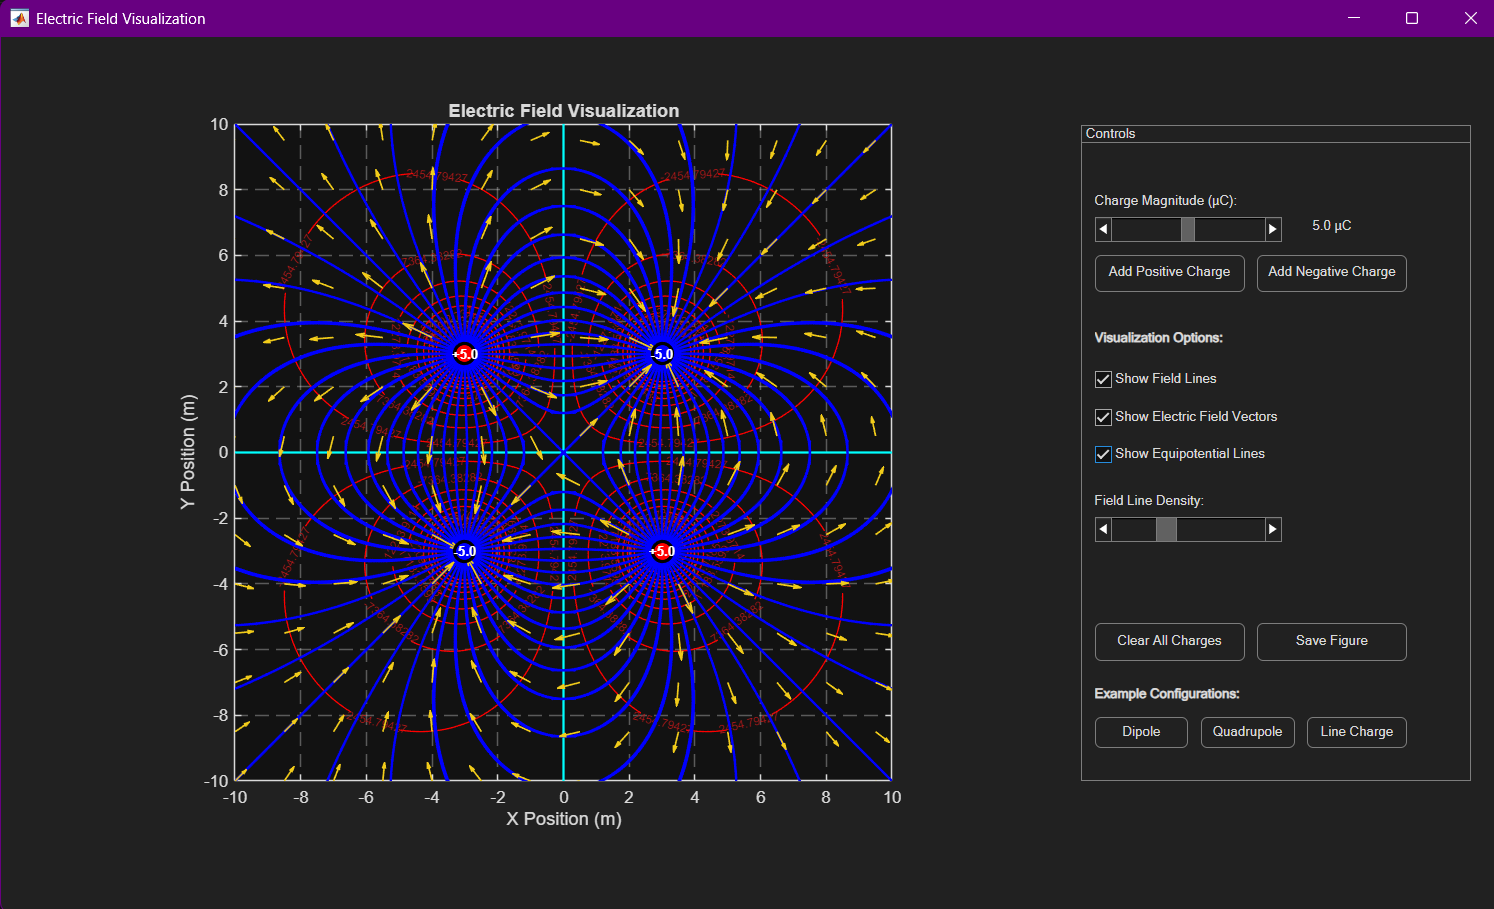
\includegraphics[width=0.8\textwidth]{../results/img/setup.png}
    \caption{The setup for simulation, including the quadrupole field example.}
\end{figure}

\begin{figure}[H]
    \centering
    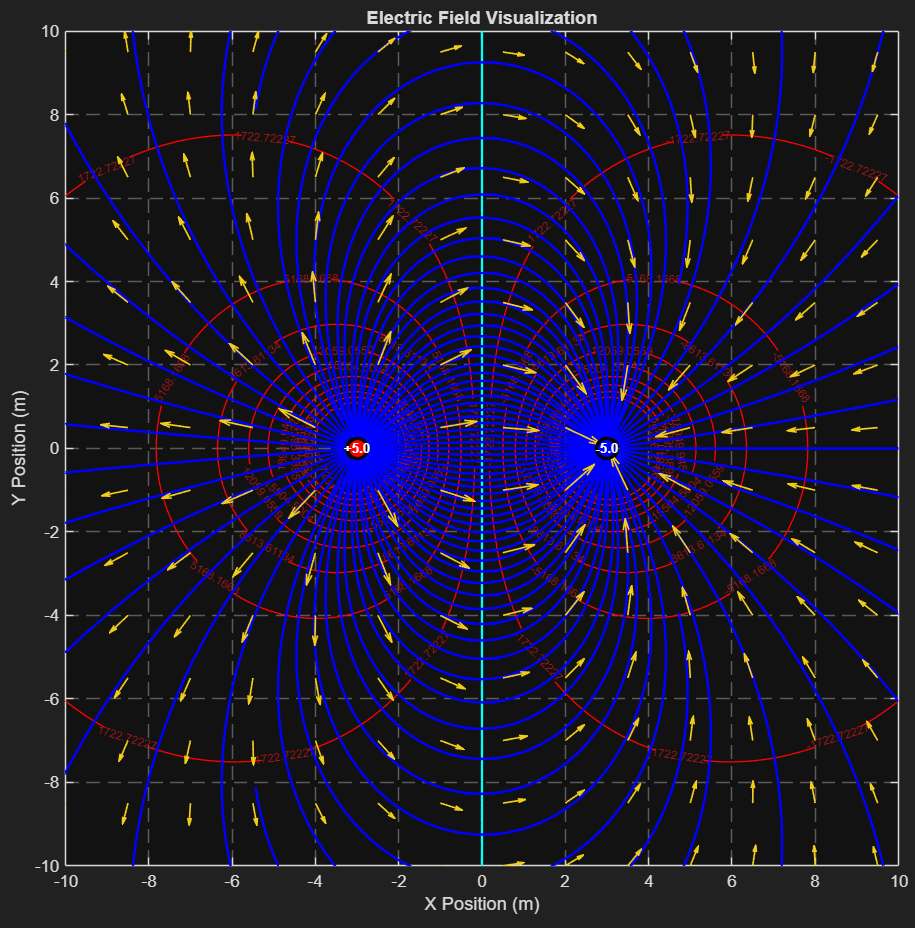
\includegraphics[width=0.8\textwidth]{../results/img/dipole.png}
    \caption{Dipole configuration: field lines (\textcolor{myblue}{blue}), equipotentials (\textcolor{myred}{red}), zero potential contour (\textcolor{mycyan}{cyan}), and field vectors (\textcolor{myyellow}{yellow}). Charges: red = positive, blue = negative.}
\end{figure}

\begin{figure}[H]
    \centering
    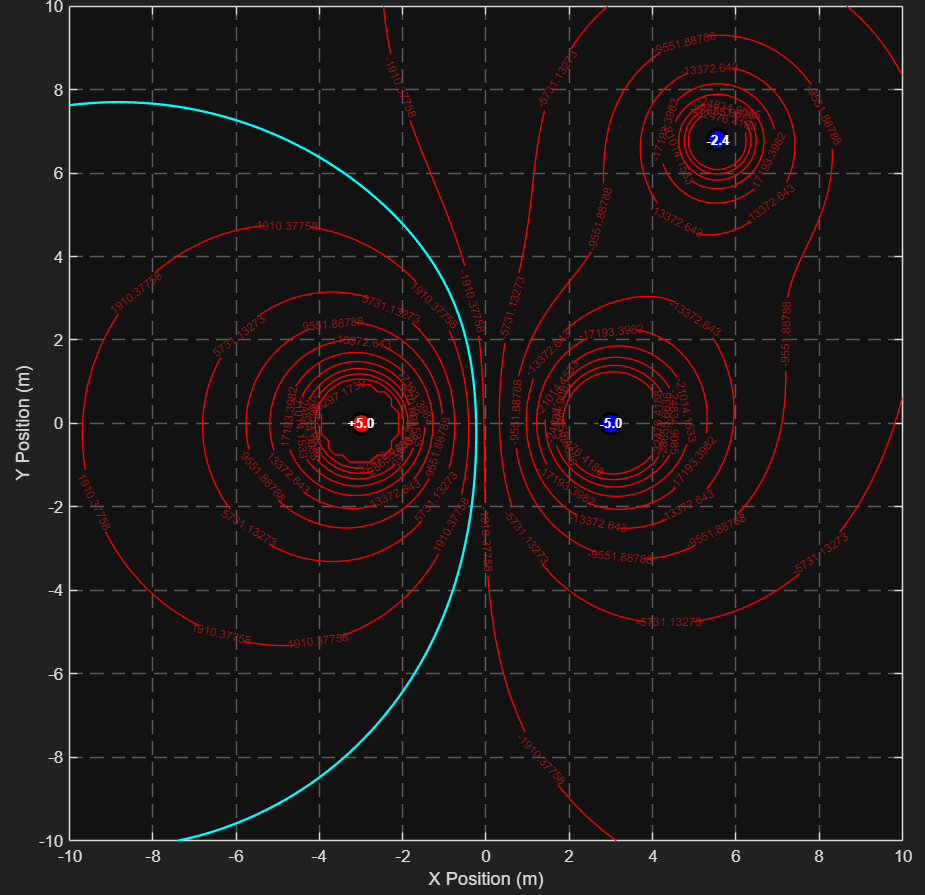
\includegraphics[width=0.8\textwidth]{../results/img/potential.png}
    \caption{Electric potential due to 3 point charges and the equipotential lines.}
\end{figure}


\begin{figure}[H]
    \centering
    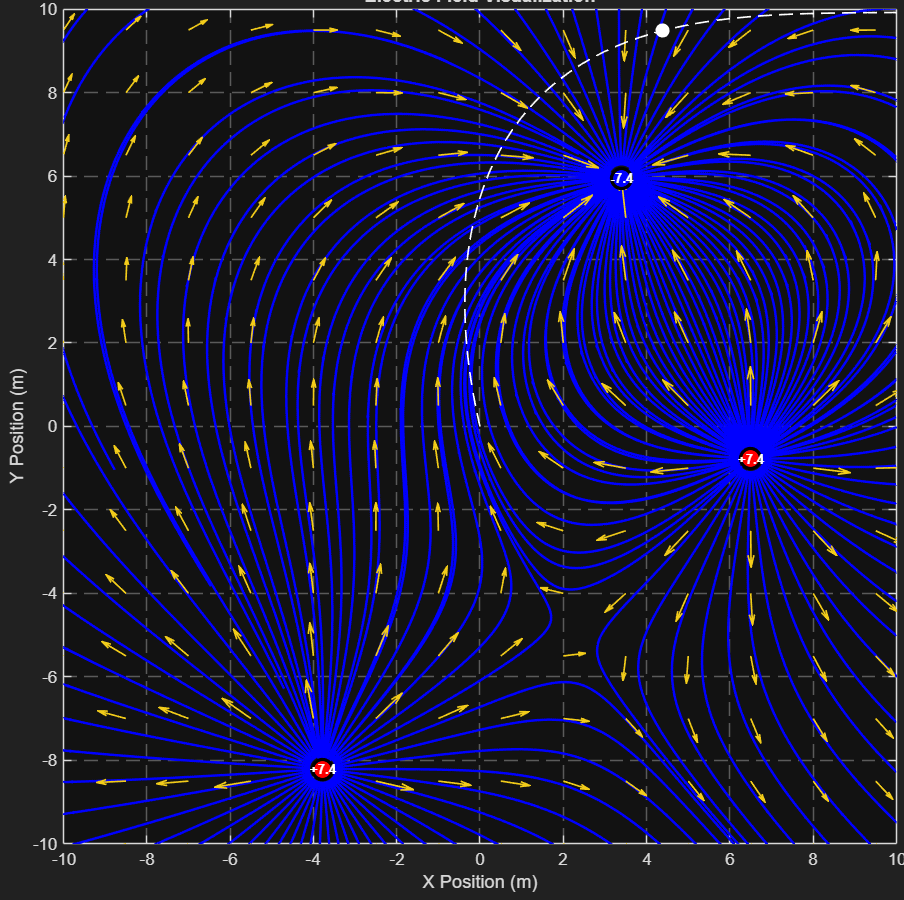
\includegraphics[width=0.8\textwidth]{../results/img/trajectory.png}
    \caption{Trajectory of the sample particle in the electric field.}
\end{figure}

\section{Discussion}
\begin{itemize}
    \item \textbf{Color conventions} improve interpretability and were chosen to maximize contrast (blue lines, yellow vectors, red equipotentials, cyan zero-potential).
    \item \textbf{RK4} is robust and preserves acceptable energy behavior for the time steps used; energy diagnostics were used to choose a stable fixed \(\Delta t\).
    \item \textbf{Symmetry and static points}: configurations with symmetric charge placement (quadrupole, uniform line) can yield zero field at the center; such points are equilibrium positions for a test particle and explain the observed lack of motion.
    \item \textbf{Dipole behavior}: despite equal magnitudes, the dipole charges produce a nonzero net field at the center in the example arrangement, which immediately accelerates a test particle starting at rest.
    \item \textbf{Regularization}: clamping small radii ($r_\text{min}$) prevents numerical blow-up but is a physical approximation; trajectories that approach charges are terminated or treated specially in the code.
\end{itemize}

\subsection{Trajectory Classification}
Based on extensive simulations, we identify five primary trajectory types: 

\paragraph{Type I - Bound Oscillatory Motion} 
Particles remain confined to a finite region, exhibiting periodic or quasi-periodic motion around equilibrium points. 

\paragraph{Type II - Spiral Trajectories} 
Particles follow spiral paths, either inward (stable spiral) or outward (unstable spiral). 

\paragraph{Type III - Escape Trajectories} 
Particles gain sufficient energy to escape to infinity, following hyperbolic-like paths. 

\paragraph{Type IV - Chaotic Motion} 
Sensitive dependence on initial conditions leads to non-repeating, irregular trajectories. 

\paragraph{Type V - Collision Trajectories} 
Particles approach source charges asymptotically (in practice, terminated when distance falls below threshold). 

\subsection{Energy Conservation Verification} 
Energy conservation provides a crucial validation of numerical accuracy: 
\begin{equation} 
    \Delta E = \frac{|E_{final} - E_{initial}|}{|E_{initial}|} < 10^{-6} 
\end{equation} 
Our simulations maintain energy conservation to within $10^{-8}$ for well-conditioned problems using RK4 integration.

\section{Improvements and Future Work} 
\subsection{Algorithmic Improvements} 

\subsubsection{Higher-Order Integration} 
Implementation of implicit methods (e.g., implicit Runge-Kutta) could improve stability for stiff problems. 

\subsubsection{Symplectic Integrators} 
Energy-conserving integration schemes would eliminate long-term drift in energy. 

\subsubsection{Adaptive Mesh Refinement} 
Dynamic grid refinement near charges could improve accuracy without excessive computational cost. 

\subsection{Physical Extensions} 

\subsubsection{Magnetic Fields} 
Including magnetic field effects would enable study of more complex particle dynamics: 
\begin{equation} 
    m\frac{d\vec{v}}{dt} = q(\vec{E} + \vec{v} \times \vec{B}) 
\end{equation} 

\subsubsection{Relativistic Effects} 
For high-energy particles, relativistic equations of motion become necessary: 
\begin{equation} 
    \frac{dp^\mu}{d\tau} = qF^{\mu\nu}u_\nu 
\end{equation} 

\subsubsection{Radiation Reaction} 
The Abraham-Lorentz force could model energy loss through electromagnetic radiation: 
\begin{equation} 
    \vec{F}_{rad} = \frac{q^2}{6\pi\epsilon_0 c^3} \frac{d^2\vec{v}}{dt^2} 
\end{equation} 

\section{Potential Issues and Limitations} 
\subsection{Numerical Instabilities} 

\subsubsection{Stiffness} 
Near charge locations, the electric field varies rapidly, leading to stiff differential equations that require small time steps for stability. 

\subsubsection{Singularities} 
The $1/r^2$ dependence of the electric field creates numerical challenges as particles approach charges. Our regularization scheme ($r_{min} = 0.1$ m) is somewhat artificial but necessary for computational stability. 

\subsubsection{Long-term Integration} 
For very long simulation times, accumulated round-off errors can lead to unphysical behavior, particularly violation of energy conservation. 

\subsection{Physical Limitations} 

\subsubsection{Classical Approximation} 
The classical treatment ignores quantum mechanical effects that become important at atomic scales or very low energies. 

\subsubsection{Point Charge Model} 
Real charges have finite size, and the point charge approximation breaks down at short distances where particle structure becomes important. 

\subsubsection{Environmental Effects} 
The simulation assumes vacuum conditions, neglecting: 
\begin{itemize} 
    \item Air resistance or medium effects 
    \item Gravitational forces 
    \item External electromagnetic fields 
    \item Interactions with other particles 
\end{itemize}

\section{Conclusions}
This project provides a clear, modular MATLAB framework to visualize electrostatic fields and to simulate test-particle motion using a fixed-step RK4 integrator. The color-coded visualizations and the GUI controls enable intuitive exploration. Important physical insights (e.g., zero-field equilibrium due to symmetry, acceleration in dipole case) are reproduced faithfully by the code.

\begin{thebibliography}{99}
    \bibitem{griffiths} D. J. Griffiths, \textit{Introduction to Electrodynamics}, 4th ed., Cambridge University Press, 2013.
    \item MathWorks Documentation: \url{https://www.mathworks.com/help/matlab/}
\end{thebibliography}

\end{document}
